\subsection{自然変換の普遍性}\label{chap-7.5-end}
  定自然変換$\natf{\varDelta f}{\varDelta A}{\varDelta B}{C}{D}$は、圏$\cat{C}$の任意の対象$C$に対して$(\varDelta f)_C=f$となる自然変換であった。一方で定関手$\varDelta A$でも$\varDelta A(C)=A$が成り立つが、この性質は定写像$\mor{\varDelta A}{\obj{C}}{\obj{D}}$によって定義されている。定自然変換と違い、関手に対象を適用する操作は対象関数で与えられているが、自然変換には与えられておらず、自然変換の成分を取る操作は写像によって定義したわけではない。\\
  自然変換を対象によって添え字付けられた射の束、と定義するのでは無く、射集合の何らかの操作によって定義できると考えたかもしれない。これは実際にエンドと呼ばれる一種の普遍性を用いることで、自然変換を再定義することができる。\\
  \begin{prop}[自然変換の普遍性]\label{prop-university-of-nat}
    圏$\cat{C}$の任意の対象$C$に対して$\cat{Set}$の射$\mor{\lambda_C}{\arset{\funccat{C}{D}}{F}{G}}{\arset{D}{FC}{GC}}$が存在し、$\cat{C}$の任意の射$\mor{f}{A}{B}$に対して、\[\arset{D}{FA}{Gf}\circ\lambda_A=\arset{D}{Ff}{GB}\circ\lambda_B\]を満たす。
    
    \begin{center}
      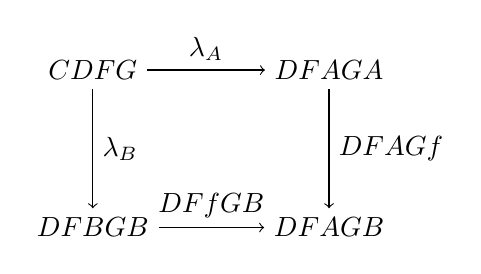
\begin{tikzpicture}[auto]
        \node (FG) at (0, 0) {$\arset{\funccat{C}{D}}{F}{G}$};
        \node (FAGA) at (3, 0) {$\arset{D}{FA}{GA}$};
        \node (FBGB) at (0, -2) {$\arset{D}{FB}{GB}$};
        \node (FAGB) at (3, -2) {$\arset{D}{FA}{GB}$};

        \draw[->] (FG) to node{$\lambda_A$}(FAGA);
        \draw[->] (FG) to node{$\lambda_B$}(FBGB);
        \draw[->] (FAGA) to node{$\arset{D}{FA}{Gf}$}(FAGB);
        \draw[->] (FBGB) to node{$\arset{D}{Ff}{GB}$}(FAGB);

      \end{tikzpicture}
    \end{center}
    
    またある対象$X$に対しても任意の対象$C$に対する$\mor{\mu_C}{\arset{\funccat{C}{D}}{F}{G}}{\arset{D}{FC}{GC}}$が存在し、\[\arset{D}{FA}{Gf}\circ\mu_A=\arset{D}{Ff}{GB}\circ\mu_B\]を満たすのであれば、
    \begin{center}
      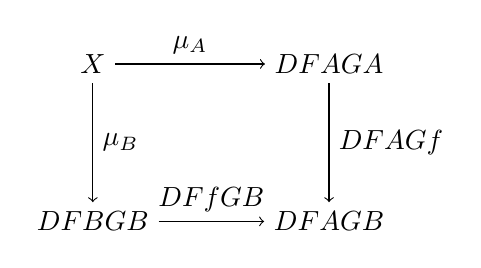
\begin{tikzpicture}[auto]
        \node (FG) at (0, 0) {$X$};
        \node (FAGA) at (3, 0) {$\arset{D}{FA}{GA}$};
        \node (FBGB) at (0, -2) {$\arset{D}{FB}{GB}$};
        \node (FAGB) at (3, -2) {$\arset{D}{FA}{GB}$};

        \draw[->] (FG) to node{$\mu_A$}(FAGA);
        \draw[->] (FG) to node{$\mu_B$}(FBGB);
        \draw[->] (FAGA) to node{$\arset{D}{FA}{Gf}$}(FAGB);
        \draw[->] (FBGB) to node{$\arset{D}{Ff}{GB}$}(FAGB);

      \end{tikzpicture}
    \end{center}
    任意の対象$C$に対して$\mu_C=\lambda_C\circ h$を満たすような射$\mor{h}{X}{\arset{\funccat{C}{D}}{F}{G}}$が一意に存在する。すなわち、$\mu_C=\lambda_C\circ h'$を満たすような$h'$が存在すれば、$h'=h$が成り立つ。
    \begin{center}
      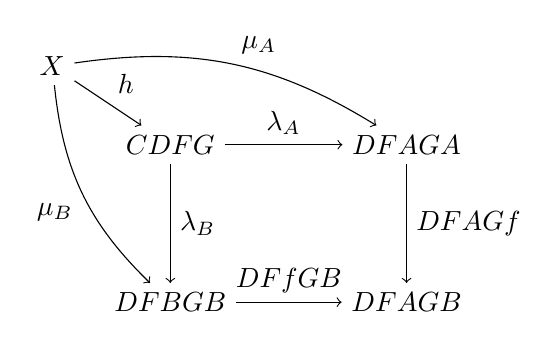
\begin{tikzpicture}[auto]
        \node (FG) at (0, 0) {$\arset{\funccat{C}{D}}{F}{G}$};
        \node (X) at (-1.5, 1) {$X$};
        \node (FAGA) at (3, 0) {$\arset{D}{FA}{GA}$};
        \node (FBGB) at (0, -2) {$\arset{D}{FB}{GB}$};
        \node (FAGB) at (3, -2) {$\arset{D}{FA}{GB}$};

        \draw[->] (FG) to node{$\lambda_A$}(FAGA);
        \draw[->] (X) to node{$h$}(FG);

        \draw[->] (FG) to node{$\lambda_B$}(FBGB);
        \draw[->,bend left = 20] (X) to node{$\mu_A$}(FAGA);
        \draw[->,bend right = 20] (X) to node[swap]{$\mu_B$}(FBGB);
        \draw[->] (FAGA) to node{$\arset{D}{FA}{Gf}$}(FAGB);
        \draw[->] (FBGB) to node{$\arset{D}{Ff}{GB}$}(FAGB);

      \end{tikzpicture}
    \end{center}
  \end{prop}
  \begin{proof}
    まず任意の対象$C$に対する$\cat{Set}$の射$\mor{\lambda_C}{\arset{\funccat{C}{D}}{F}{G}}{\arset{D}{FC}{GC}}$を定義する。\\
    任意の自然変換$\nat{\alpha}{F}{G}$に対して$\lambda_C(\alpha)=\alpha_C$とする。任意の自然変換はある対象に対する成分をただ一つ持つから、この操作は写像であり、$\cat{Set}$の射である。すると、
    \begin{align*}
      \arset{D}{FA}{Gf}\circ\lambda_A(\alpha)&=\arset{D}{FA}{Gf}(\alpha_A)&\text{($\lambda$の定義)}\\
      &=Gf\circ\alpha_A&\text{(射写像の定義)}\\
      \arset{D}{Ff}{GB}\circ\lambda_B(\alpha)&=\arset{D}{Ff}{GB}(\alpha_B)&\text{($\lambda$の定義)}\\
      &=\alpha_B\circ Ff&\text{(射写像の定義)}
    \end{align*}
  であり、$\alpha$の自然性から$Gf\circ\alpha_A=\alpha_B\circ Ff$が成り立つ。よって$\arset{D}{FA}{Gf}\circ\lambda_A=\arset{D}{Ff}{GB}\circ\lambda_B$を満たす。\\
  この等式では自然変換の成分が写像で与えられた場合の自然性を射写像を用いて課していることが分かる。\\
  次に射$h$の存在と一意性を示そうと思う。そこでまずは任意の対象$X$に終対象$1$を当てはめて考える。射$\mor{\mu_C}{1}{\arset{D}{FC}{GC}}$は射$\mor{\mu_A}{FA}{GA}$であり、任意の対象$C$に対して存在する。更に仮定より$\arset{D}{FA}{Gf}\circ\mu_A=\arset{D}{Ff}{GB}\circ\mu_B$が成り立つ。
  \begin{align*}
    \arset{D}{FA}{Gf}\circ\mu_A&=\arset{D}{Ff}{GB}\circ\mu_B\\
    \arset{D}{FA}{Gf}(\mu_A)&=\arset{D}{Ff}{GB}(\mu_B)&\text{(元と終対象からの射の同一視)}\\
    Gf\circ\mu_A&=\mu_B\circ Ff&\text{(射写像の定義)}
  \end{align*}
  よって自然変換の定義より、$\mu_C$は対象$C$成分であることが分かる。この自然変換を$\nat{\mu}{F}{G}$とすると、$\mu$は$\arset{\funccat{C}{D}}{F}{G}$の元である。すなわち$\mor{\mu}{1}{\arset{\funccat{C}{D}}{F}{G}}$と表せる。ここで$h=\mu$とすると$\lambda$は成分を取る写像であったから、$\mu_C=\lambda_C(\mu)=\lambda_C\circ\mu=\lambda_C\circ h$が成り立つ。
  \begin{center}
    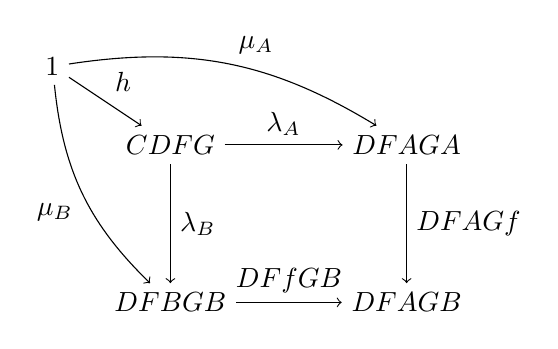
\begin{tikzpicture}[auto]
      \node (FG) at (0, 0) {$\arset{\funccat{C}{D}}{F}{G}$};
      \node (X) at (-1.5, 1) {$1$};
      \node (FAGA) at (3, 0) {$\arset{D}{FA}{GA}$};
      \node (FBGB) at (0, -2) {$\arset{D}{FB}{GB}$};
      \node (FAGB) at (3, -2) {$\arset{D}{FA}{GB}$};

      \draw[->] (FG) to node{$\lambda_A$}(FAGA);
      \draw[->] (X) to node{$h$}(FG);

      \draw[->] (FG) to node{$\lambda_B$}(FBGB);
      \draw[->,bend left = 20] (X) to node{$\mu_A$}(FAGA);
      \draw[->,bend right = 20] (X) to node[swap]{$\mu_B$}(FBGB);
      \draw[->] (FAGA) to node{$\arset{D}{FA}{Gf}$}(FAGB);
      \draw[->] (FBGB) to node{$\arset{D}{Ff}{GB}$}(FAGB);
    \end{tikzpicture}
  \end{center}
  一意性に関しても、$\mu_C=\lambda_C\circ h'$であるような$h'$が存在したとしても、$\mu_C={h'}_C$であり、自然変換の定義から$h'=\mu=h$が成り立つ。\\
  次に対象$1$を任意の対象$X$に拡張しよう。$X$の任意の元$x$に対し$\mu_C(x)$はある自然変換の$C$成分である。上記の議論から自然変換$h(x)_C=\mu_C(x)$であるため、自然変換$h(x)$は任意の$x$に対して一意に存在することになる。よって条件を満たす$h$は存在する。
  一意性に関しても、$\mor{h'}{\arset{\funccat{C}{D}}{F}{G}}{\arset{D}{FA}{GA}}$が存在して\[\lambda_C\circ h' = \mu_C\]が成り立ったとしても、任意の元$x$に対して\[\lambda_C\circ h'(x) = \mu_C(x)\]が成り立つから、$h'(x)=h(x)$となる。よって$h = h'$であり、一意性が示せた。

  \begin{center}
    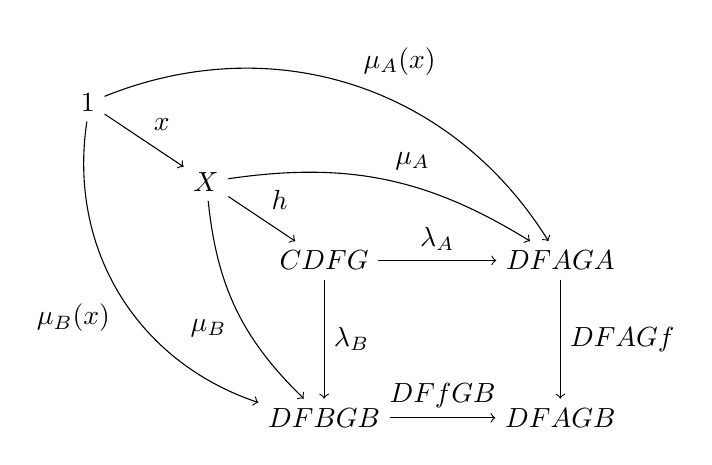
\begin{tikzpicture}[auto]
      \node (FG) at (0, 0) {$\arset{\funccat{C}{D}}{F}{G}$};
      \node (X) at (-1.5, 1) {$X$};
      \node (1) at (-3, 2) {$1$};
      \node (FAGA) at (3, 0) {$\arset{D}{FA}{GA}$};
      \node (FBGB) at (0, -2) {$\arset{D}{FB}{GB}$};
      \node (FAGB) at (3, -2) {$\arset{D}{FA}{GB}$};
      \draw[->] (FG) to node{$\lambda_A$}(FAGA);
      \draw[->] (X) to node{$h$}(FG);
      \draw[->] (1) to node{$x$}(X);
      \draw[->] (FG) to node{$\lambda_B$}(FBGB);
      \draw[->,bend left = 20] (X) to node{$\mu_A$}(FAGA);
      \draw[->,bend right = 20] (X) to node[swap]{$\mu_B$}(FBGB);
      \draw[->,bend left = 40] (1) to node{$\mu_A(x)$}(FAGA);
      \draw[->,bend right = 40] (1) to node[swap]{$\mu_B(x)$}(FBGB);
      \draw[->] (FAGA) to node{$\arset{D}{FA}{Gf}$}(FAGB);
      \draw[->] (FBGB) to node{$\arset{D}{Ff}{GB}$}(FAGB);
    \end{tikzpicture}
    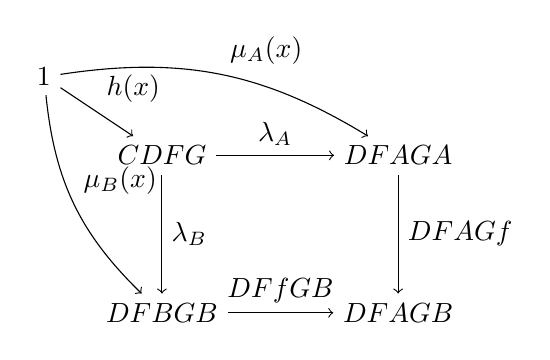
\begin{tikzpicture}[auto]
      \node (FG) at (0, 0) {$\arset{\funccat{C}{D}}{F}{G}$};
      \node (X) at (-1.5, 1) {$1$};
      \node (FAGA) at (3, 0) {$\arset{D}{FA}{GA}$};
      \node (FBGB) at (0, -2) {$\arset{D}{FB}{GB}$};
      \node (FAGB) at (3, -2) {$\arset{D}{FA}{GB}$};
      \draw[->] (FG) to node{$\lambda_A$}(FAGA);
      \draw[->] (X) to node{$h(x)$}(FG);
      \draw[->] (FG) to node{$\lambda_B$}(FBGB);
      \draw[->,bend left = 20] (X) to node{$\mu_A(x)$}(FAGA);
      \draw[->,bend right = 20] (X) to node{$\mu_B(x)$}(FBGB);
      \draw[->] (FAGA) to node{$\arset{D}{FA}{Gf}$}(FAGB);
      \draw[->] (FBGB) to node{$\arset{D}{Ff}{GB}$}(FAGB);
    \end{tikzpicture}
  \end{center}
\end{proof}
  \begin{define}[エンド]\label{def-end}
    ある圏$\cat{C,D}$と、関手$\functor{F}{C^{op}\times C}{D}$に対するエンド$(\cend{C}{C} F(C,C),\lambda)$を以下のように構成する。
    \begin{quote}
      \begin{mydescription}
        \item[楔]楔と呼ばれる組$(X,\mu)$を以下のように構成する。圏$\cat{D}$の対象である$X$と圏$\cat{C}$の任意の対象$C$に対して$\mor{\mu}{X}{T(C,C)}$なる射が存在して、圏$\cat{C}$の任意の射$\mor{f}{A}{B}$に対して$F(A,f)\circ\mu_A=F(f,B)\circ\mu_B$が成り立つとする。
        \begin{center}
          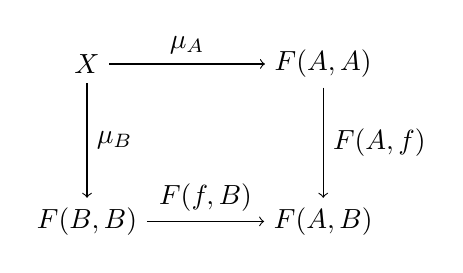
\begin{tikzpicture}[auto]
            \node (FG) at (0, 0) {$X$};
            \node (FAGA) at (3, 0) {$F(A,A)$};
            \node (FBGB) at (0, -2) {$F(B,B)$};
            \node (FAGB) at (3, -2) {$F(A,B)$};
    
            \draw[->] (FG) to node{$\mu_A$}(FAGA);  
            \draw[->] (FG) to node{$\mu_B$}(FBGB);
            \draw[->] (FAGA) to node{$F(A,f)$}(FAGB);
            \draw[->] (FBGB) to node{$F(f,B)$}(FAGB);
          \end{tikzpicture}
        \end{center}

        \item[普遍性] 関手$F$に対してある楔$(\cend{C}{C} F(C,C),\lambda)$がエンドであるとは、他の楔$(X,\mu)$に対して、$\mu_C = \lambda_C\circ h$が成り立つような$\mor{h}{X}{\cend{C}{C}F(C,C)}$が一意に存在する時である。
        \begin{center}
          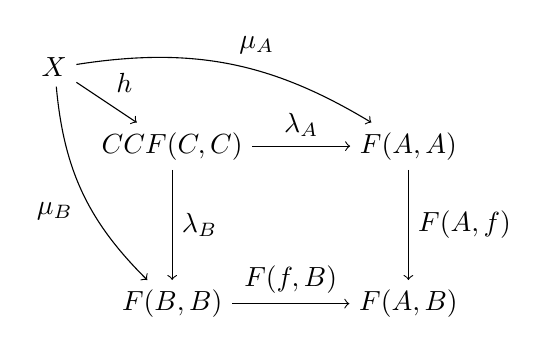
\begin{tikzpicture}[auto]
            \node (FG) at (0, 0) {$\cend{C}{C} F(C,C)$};
            \node (X) at (-1.5, 1) {$X$};
            \node (FAGA) at (3, 0) {$F(A,A)$};
            \node (FBGB) at (0, -2) {$F(B,B)$};
            \node (FAGB) at (3, -2) {$F(A,B)$};
    
            \draw[->] (FG) to node{$\lambda_A$}(FAGA);
            \draw[->] (X) to node{$h$}(FG);
    
            \draw[->] (FG) to node{$\lambda_B$}(FBGB);
            \draw[->,bend left = 20] (X) to node{$\mu_A$}(FAGA);
            \draw[->,bend right = 20] (X) to node[swap]{$\mu_B$}(FBGB);
            \draw[->] (FAGA) to node{$F(A,f)$}(FAGB);
            \draw[->] (FBGB) to node{$F(f,B)$}(FAGB);
          \end{tikzpicture}
        \end{center}
      \end{mydescription}
    \end{quote}
  \end{define}
  エンドの定義から自然変換の射集合は明らかにエンドである。
  \begin{prop}
    $\arset{\funccat{C}{D}}{F}{G}=\cend{C}{C}\arset{D}{FC}{GC}$
  \end{prop}

  \begin{prop}[エンドの一意性]
    関手$F$におけるエンド$(\cend{C}{C}F(C,C),\lambda)$に対して、同様に関手$F$に対するエンド$(X,\mu)$が存在するとする。この時$X\cong\cend{C}{C}F(C,C)$が成り立つ。
  \end{prop}
  \begin{proof}
    $(\cend{C}{C}F(C,C),\lambda)$と$(X,\mu)$はどちらも$F$に対する楔であるから、$\mor{h}{\cend{C}{C}F(C,C)}{X}$、$\mor{h^{-1}}{X}{\cend{C}{C}F(C,C)}$なる一意に定まる射が存在する。これらが同型射であることを調べれば良い。

    エンドの普遍性より、
    \begin{align*}
      \mu_C\circ(h'\circ h) &=(\mu_C\circ h')\circ h\\
      &= \lambda_C \circ h\\
      &=\mu_C\\
    \end{align*}
    となるが、$\mor{id_X}{X}{X}$もまた$\mu_C\circ id_X = \mu_C$を満たす。すると$X$のエンドの普遍性により、このような射は一意に定まるから$h'\circ h=id_X$である。
    \begin{center}
      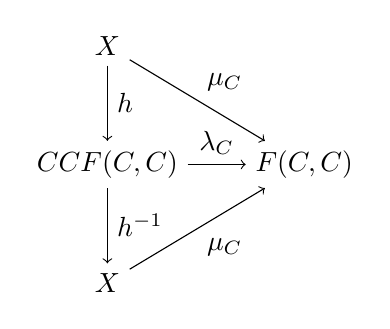
\begin{tikzpicture}[auto]
        \node (X) at (0, 0) {$X$};
        \node (end) at (0, -1.5) {$\cend{C}{C}F(C,C)$};
        \node (X2) at (0, -3) {$X$};
        \node (fcc) at (2.5, -1.5) {$F(C,C)$};
        \draw[->] (X) to node{$h$}(end);
        \draw[->] (end) to node{$h^{-1}$}(X2);
        \draw[->] (X) to node{$\mu_C$}(fcc);
        \draw[->] (X2) to node[swap]{$\mu_C$}(fcc);
        \draw[->] (end) to node{$\lambda_C$}(fcc);
      \end{tikzpicture}
    \end{center}
    同様に$h\circ h'=id$であるから$X\cong\cend{C}{C}F(C,C)$である。
  \end{proof}
  またこの命題の逆もまた成り立つ。
  \begin{prop}[同型のエンドの保存]
    エンド$(\cend{C}{C}F(C,C),\lambda)$に対して$X\cong \cend{C}{C}F(C,C)$であれば、$X$もまた$F$に対するエンドとなる。
  \end{prop}
  \begin{proof}
    同型射を$\mor{i}{X}{\cend{C}{C}F(C,C)},\ \mor{i^{-1}}{\cend{C}{C}F(C,C)}{X}$とする。この時$\mor{\lambda_C\circ i}{X}{F(C,C)}$が楔の定義を満たすかどうかを確認する。すなわち
    \[F(A,f)\circ\lambda_A\circ i=F(f,B)\circ\lambda_B\circ i\]が成り立てば良いが、これは明らかに\[F(A,f)\circ\lambda_A=F(f,B)\circ\lambda_B\]より成り立つ。
    \begin{center}
      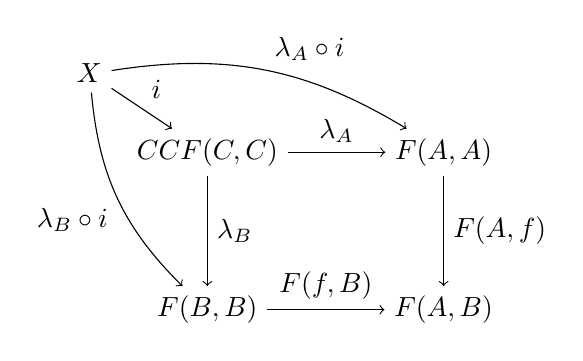
\begin{tikzpicture}[auto]
        \node (FG) at (0, 0) {$\cend{C}{C} F(C,C)$};
        \node (X) at (-1.5, 1) {$X$};
        \node (FAGA) at (3, 0) {$F(A,A)$};
        \node (FBGB) at (0, -2) {$F(B,B)$};
        \node (FAGB) at (3, -2) {$F(A,B)$};

        \draw[->] (FG) to node{$\lambda_A$}(FAGA);
        \draw[->] (X) to node{$i$}(FG);

        \draw[->] (FG) to node{$\lambda_B$}(FBGB);
        \draw[->,bend left = 20] (X) to node{$\lambda_A\circ i$}(FAGA);
        \draw[->,bend right = 20] (X) to node[swap]{$\lambda_B\circ i$}(FBGB);
        \draw[->] (FAGA) to node{$F(A,f)$}(FAGB);
        \draw[->] (FBGB) to node{$F(f,B)$}(FAGB);
      \end{tikzpicture}
    \end{center}

    次に$F$に対する任意の楔$(Y,\mu)$に対して普遍性が成り立つかを調べる。
    まずエンドの普遍性から$\lambda_C\circ h = \mu_C$なる射$\mor{h}{Y}{\cend{C}{C}F(C,C)}$が一意に存在する。

    $X$をエンドであるならば、同様の条件を満たす射が一意に存在する必要があるが、それを$\mor{i^{-1}\circ h}{Y}{X}$とする。すると、
    \[\mu_C=\lambda_C\circ h = \lambda_C\circ i\circ i^{-1}\circ h =(\lambda_C\circ i)\circ (i^{-1}\circ h)\]となり、そのような射の存在は示せた。
    \begin{center}
      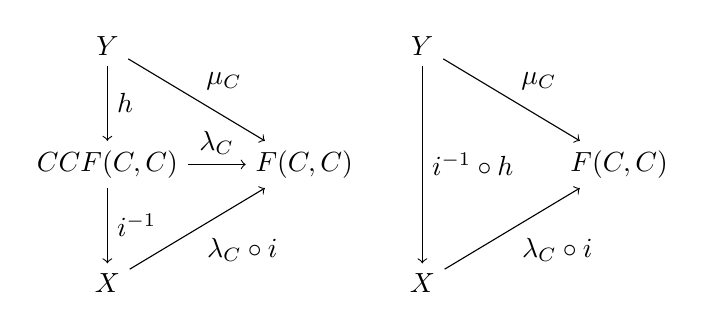
\begin{tikzpicture}[auto]
        \node (X) at (0, 0) {$Y$};
        \node (end) at (0, -1.5) {$\cend{C}{C}F(C,C)$};
        \node (X2) at (0, -3) {$X$};
        \node (fcc) at (2.5, -1.5) {$F(C,C)$};
        \draw[->] (X) to node{$h$}(end);
        \draw[->] (end) to node{$i^{-1}$}(X2);
        \draw[->] (X) to node{$\mu_C$}(fcc);
        \draw[->] (X2) to node[swap]{$\lambda_C\circ i$}(fcc);
        \draw[->] (end) to node{$\lambda_C$}(fcc);

        \node (X) at (4, 0) {$Y$};
        \node (X2) at (4, -3) {$X$};
        \node (fcc) at (6.5, -1.5) {$F(C,C)$};
        \draw[->] (X) to node{$i^{-1}\circ h$}(X2);
        \draw[->] (X) to node{$\mu_C$}(fcc);
        \draw[->] (X2) to node[swap]{$\lambda_C\circ i$}(fcc);
      \end{tikzpicture}
    \end{center}
    また$\mu_C =(\lambda_C\circ i)\circ (i^{-1}\circ h')$を満たすような射$h'$が存在しても、$\mu_C=\lambda_C\circ h'$が直ちに成り立つからエンドの普遍性より$h=h'$となり、$i^{-1}\circ h=i^{-1}\circ h'$もまた成り立つ。よって$i^{-1}\circ h$が一意に存在することを示せたから$X$はエンドになる。
  \end{proof}
